% ============================================================
% Seccion: Resultados preliminares
% Etapa 3 (GMM y MCDSVDD) y etapa 4 (curvas de luz y outliers)
% Todas las metricas son del conjunto de test
% Figuras: figures/gmm.png, mcdsvdd.png, prototipos.png, outliers.png
% ============================================================
\section{Resultados preliminares}

% ============================================================
\begin{frame}
\frametitle{Etapa 3: clustering con mezcla de gaussianas (GMM)}
\vspace{-0.8em}
\begin{center}
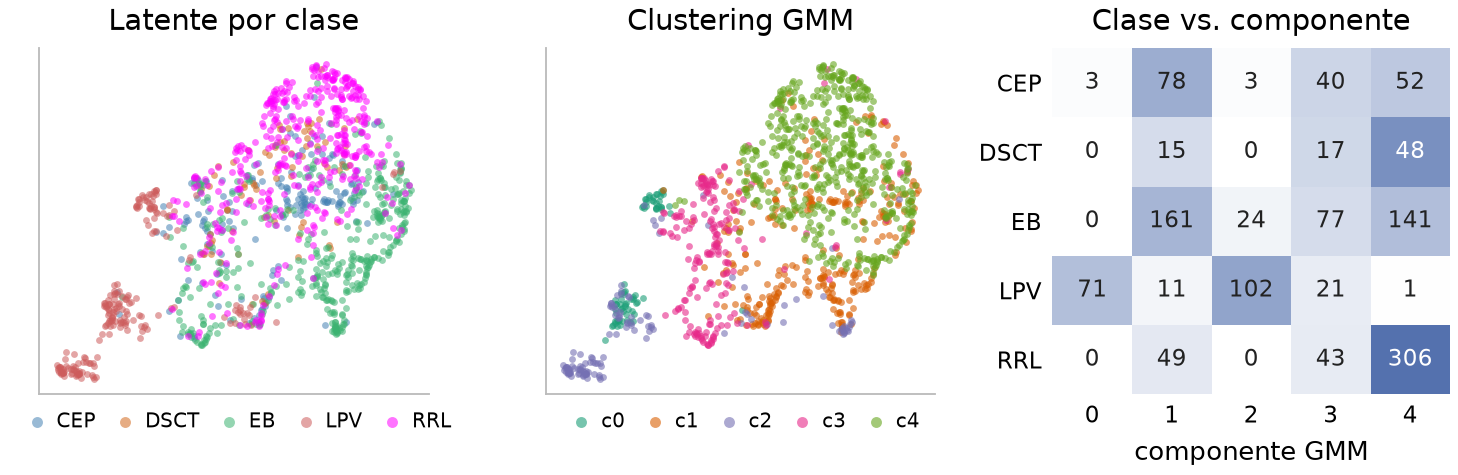
\includegraphics[width=0.78\textwidth]{figures/gmm.png}\\[-0.2em]
{\scriptsize UMAP del latente en test (\texttt{n\_neighbors} = 20). El GMM agrupa en las 8
dimensiones, no sobre el UMAP}
\end{center}
\vspace{-0.7em}
\begin{columns}[T]
\begin{column}{0.50\textwidth}
{\footnotesize \textbf{Decisiones}
\begin{itemize}\itemsep=2pt
\item 5 componentes, uno por clase, para comparar con las etiquetas (el BIC prefiere 10)
\item Covarianza completa. Se ajusta solo con el latente de train y sin etiquetas, que solo
  sirven para medir
\end{itemize}
}
\end{column}

\begin{column}{0.47\textwidth}
{\footnotesize \textbf{Resultado en test}: \textcolor{structure}{\textbf{ARI 0,20 \quad NMI 0,26}}
\begin{itemize}\itemsep=2pt
\item Recupera LPV: 173 de 206 caen en dos componentes casi puros
\item CEP, DSCT, EB y RRL quedan mezcladas: sin etiquetas, el latente no las separa
\end{itemize}
}
\end{column}
\end{columns}
\end{frame}

% ============================================================
\begin{frame}
\frametitle{Etapa 3: clustering con Multi-Class Deep SVDD}
\vspace{-0.8em}
\begin{center}
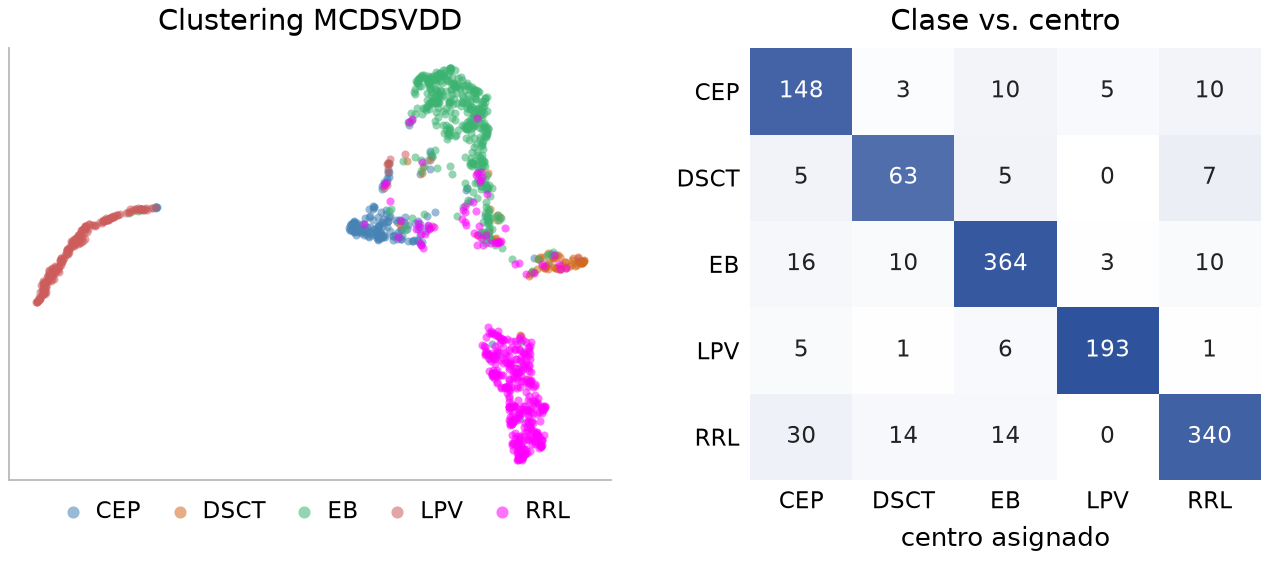
\includegraphics[width=0.66\textwidth]{figures/mcdsvdd.png}\\[-0.2em]
{\scriptsize UMAP del latente de MCDSVDD en test (\texttt{n\_neighbors} = 20)}
\end{center}
\vspace{-0.8em}
\begin{columns}[T]
\begin{column}{0.50\textwidth}
{\footnotesize \textbf{Decisiones}
\begin{itemize}\itemsep=1pt
\item Parte del encoder ya entrenado. Cada clase tiene un centro fijo y la pérdida es la
  distancia a él
\item Tasa $10^{-4}$ y 25 épocas, aún sin ajuste fino
\item \textbf{Sobremuestreo} de las clases chicas, solo en train
\end{itemize}
}
\end{column}

\begin{column}{0.47\textwidth}
{\footnotesize \textbf{Resultado en test}: \textcolor{structure}{\textbf{ARI 0,73 \quad NMI 0,67}}
\begin{itemize}\itemsep=2pt
\item Las cinco clases quedan mayormente en su centro
\item El sobremuestreo sube el ARI de 0,69 a 0,73, y DSCT pasa de 26 a 63 de 80 objetos en su
  centro
\end{itemize}
}
\end{column}
\end{columns}
\end{frame}

% ============================================================
\begin{frame}
\frametitle{Etapa 4: curvas de luz de los prototipos}
\vspace{-0.8em}
\begin{center}
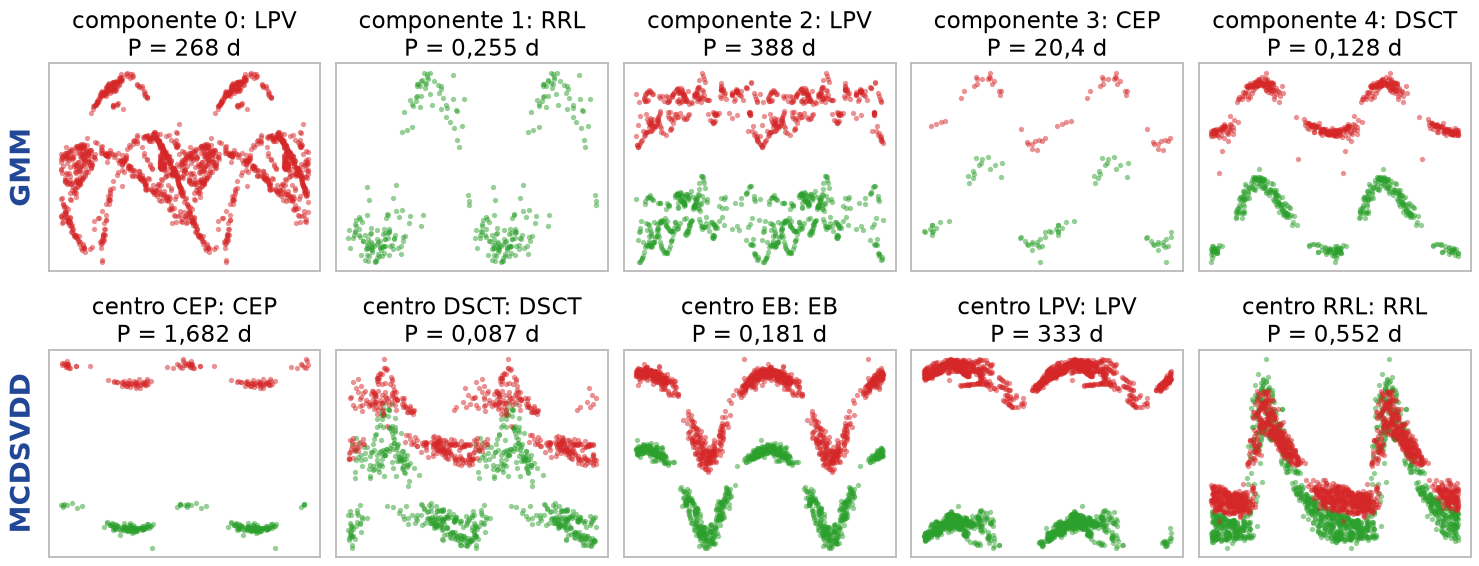
\includegraphics[width=0.93\textwidth]{figures/prototipos.png}\\[-0.1em]
{\scriptsize Prototipo: el objeto de test más cercano al centro de cada grupo. Curvas plegadas
con el período multibanda}
\end{center}
\vspace{-0.5em}
{\footnotesize
\begin{itemize}\itemsep=2pt
\item \textbf{GMM}: los componentes 0 y 2 agrupan estrellas LPV. Los componentes 1, 3 y 4
  mezclan varias clases de período corto, y por eso su prototipo puede ser de cualquiera de ellas
\item \textbf{MCDSVDD}: cada centro muestra la curva típica de su clase
\end{itemize}
}
\end{frame}

% ============================================================
\begin{frame}
\frametitle{Etapa 4: análisis de outliers}
\vspace{-0.8em}
\begin{center}
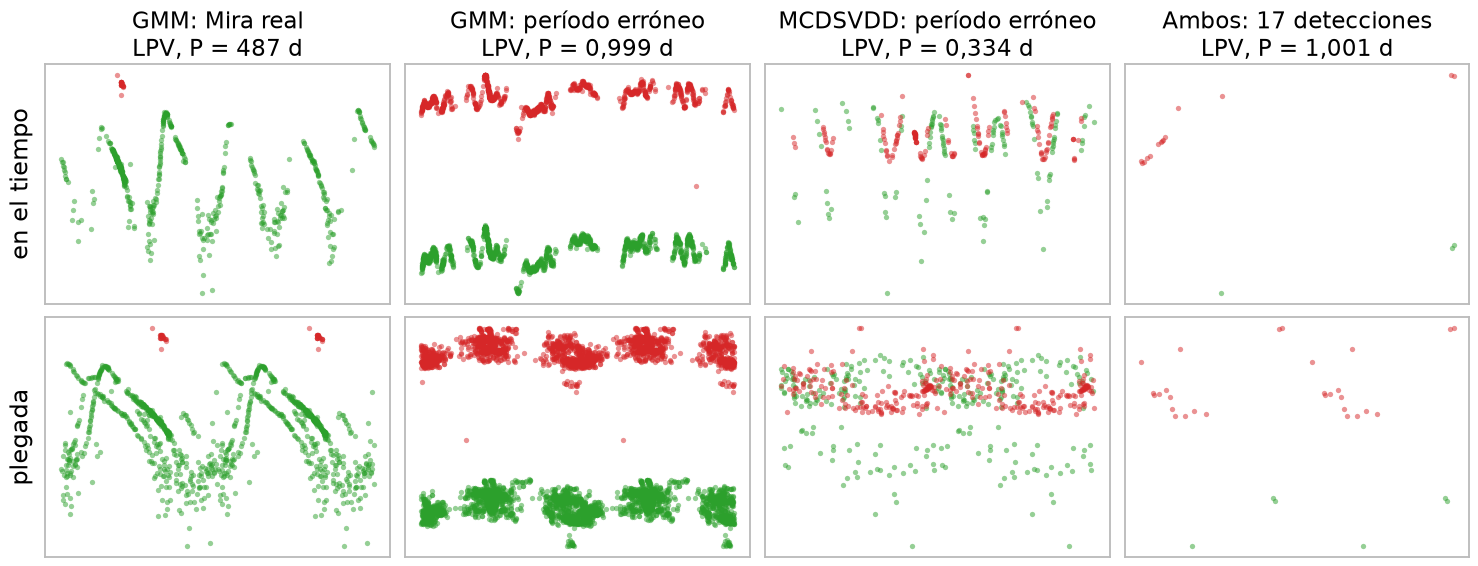
\includegraphics[width=0.90\textwidth]{figures/outliers.png}
\end{center}
\vspace{-0.6em}
{\footnotesize
\begin{itemize}\itemsep=2pt
\item \textbf{GMM} (menor verosimilitud): 5 de los 6 más extremos son LPV. Hay Miras reales de
  gran amplitud y otras con el período mal calculado
\item \textbf{MCDSVDD} (mayor distancia a los centros): objetos con pocas detecciones o con el
  período mal calculado
\item \textbf{Hallazgo}: varios outliers no son estrellas raras, sino objetos con datos malos
\end{itemize}
}
\end{frame}
